\chapter{Forecasting Results}
\label{ch:forecasting}

\section{Consumption Forecasting}

Table~\ref{tab:consumption_models} compares model performance on the validation set.

\begin{table}[H]
\centering
\caption{Consumption forecasting model comparison (validation set).}
\label{tab:consumption_models}
\begin{tabular}{lrrrr}
\toprule
\textbf{Model} & \textbf{MAE (W)} & \textbf{RMSE (W)} & \textbf{MAPE (\%)} & $\mathbf{R^2}$ \\
\midrule
Naive Baseline & 521.8 & 882.1 & 53.9 & 0.0616 \\
Linear Regression & 108.1 & 183.9 & 16.3 & 0.9592 \\
Random Forest & 47.9 & 167.7 & 4.1 & 0.9661 \\
\textbf{XGBoost} & \textbf{49.3} & \textbf{153.5} & \textbf{4.0} & \textbf{0.9716} \\
\bottomrule
\end{tabular}
\end{table}

XGBoost achieves the lowest RMSE (153.5~W) and highest $R^2$ (0.9716). On the unseen test set, performance improves further: MAE~=~38.0~W, RMSE~=~73.1~W, $R^2$~=~0.9941, MAPE~=~3.3\%. The improvement on the test set is expected because the test period (spring/early summer) has more regular consumption patterns than the validation period (late winter).

\begin{figure}[H]
    \centering
    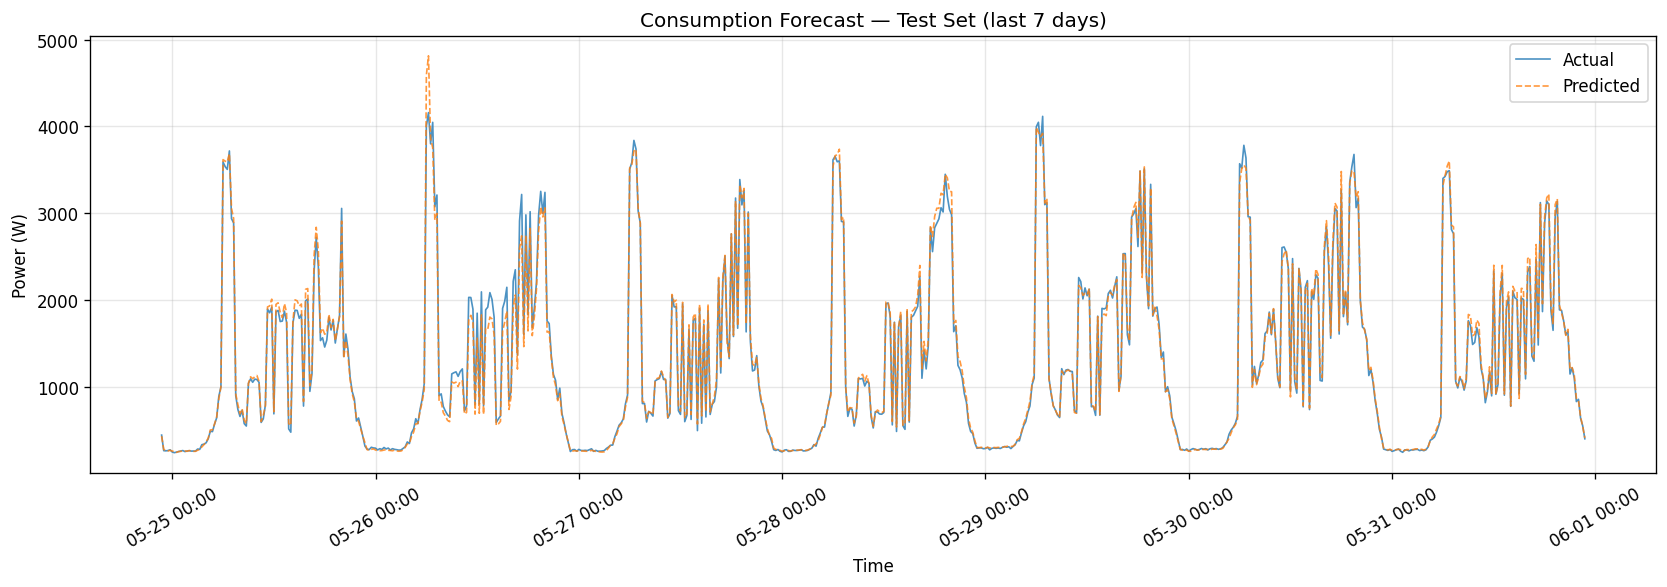
\includegraphics[width=\textwidth]{figures/consumption_forecast_test.png}
    \caption{Actual vs predicted consumption --- test set (last 7 days).}
    \label{fig:consumption_forecast}
\end{figure}

\begin{figure}[H]
    \centering
    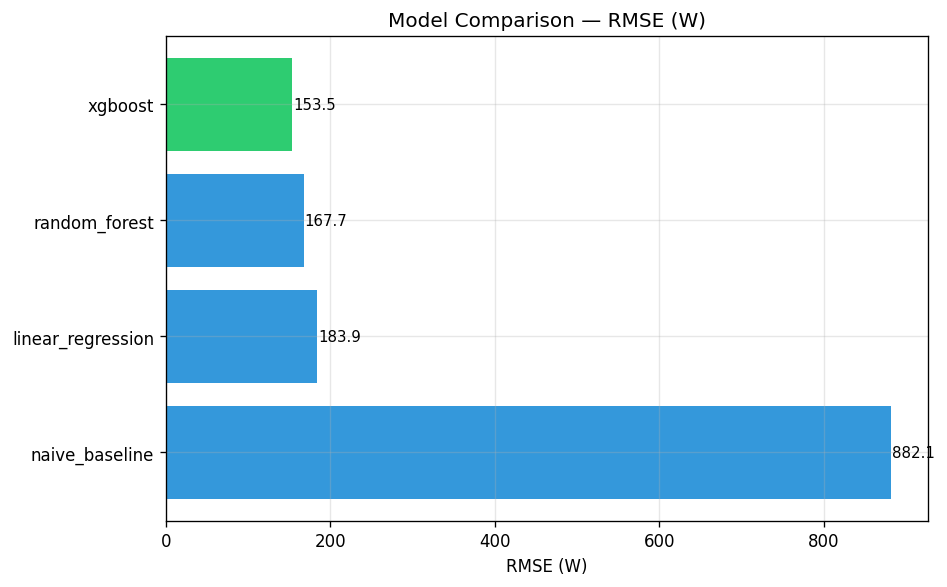
\includegraphics[width=0.75\textwidth]{figures/consumption_model_rmse.png}
    \caption{Consumption model comparison by RMSE.}
    \label{fig:consumption_rmse}
\end{figure}

\begin{figure}[H]
    \centering
    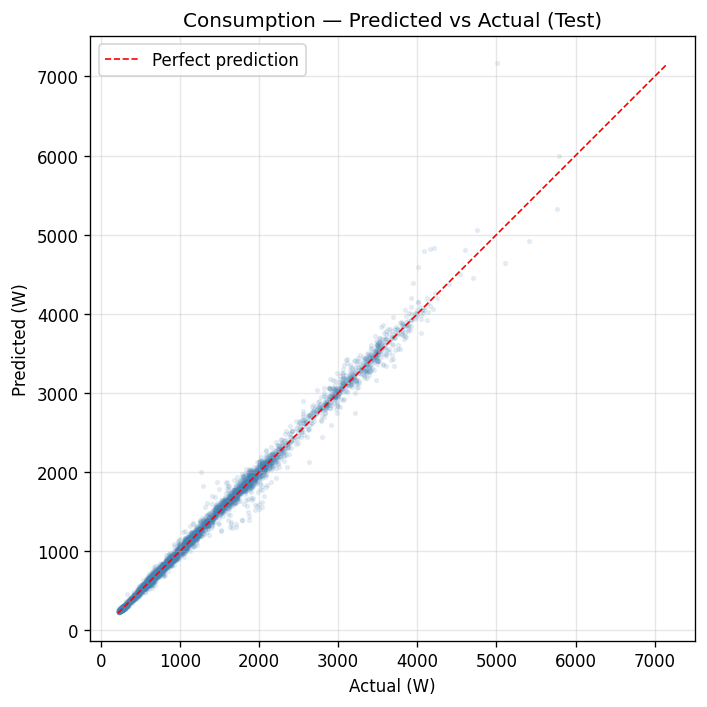
\includegraphics[width=0.6\textwidth]{figures/consumption_scatter.png}
    \caption{Predicted vs actual consumption scatter plot (test set).}
    \label{fig:consumption_scatter}
\end{figure}

The naive baseline's poor performance ($R^2 = 0.06$) confirms that simple historical averages are inadequate for this building's variable consumption profile, justifying the use of ML models.

\section{PV Production Forecasting}

All three ML models achieve near-perfect performance on the synthetic PV data ($R^2 > 0.999$). This is expected because synthetic PV power is a deterministic function of irradiance and temperature, both of which are direct features. With real-world data, cloud variability, dust accumulation, and partial shading would introduce prediction errors, and $R^2$ values of 0.85--0.95 would be expected.

\begin{figure}[H]
    \centering
    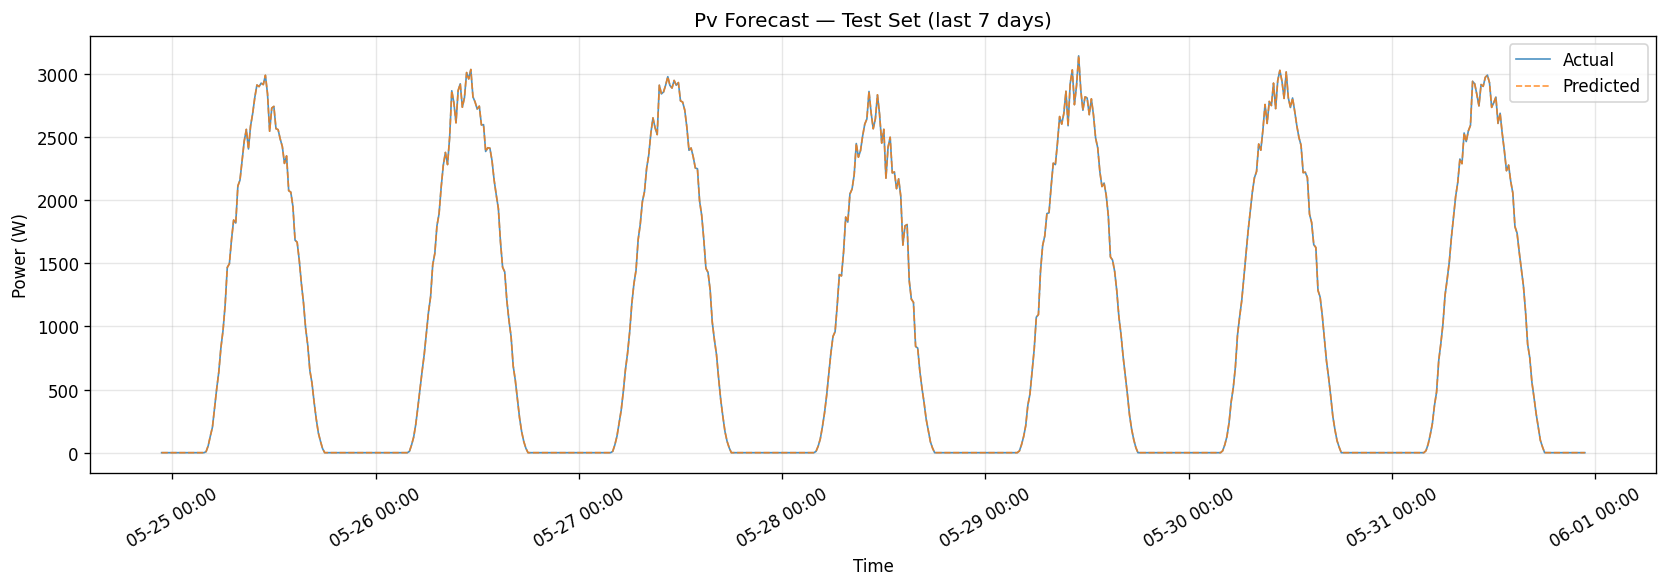
\includegraphics[width=\textwidth]{figures/pv_forecast_test.png}
    \caption{Actual vs predicted PV production --- test set (last 7 days).}
    \label{fig:pv_forecast}
\end{figure}

\section{Feature Importance}

\begin{figure}[H]
    \centering
    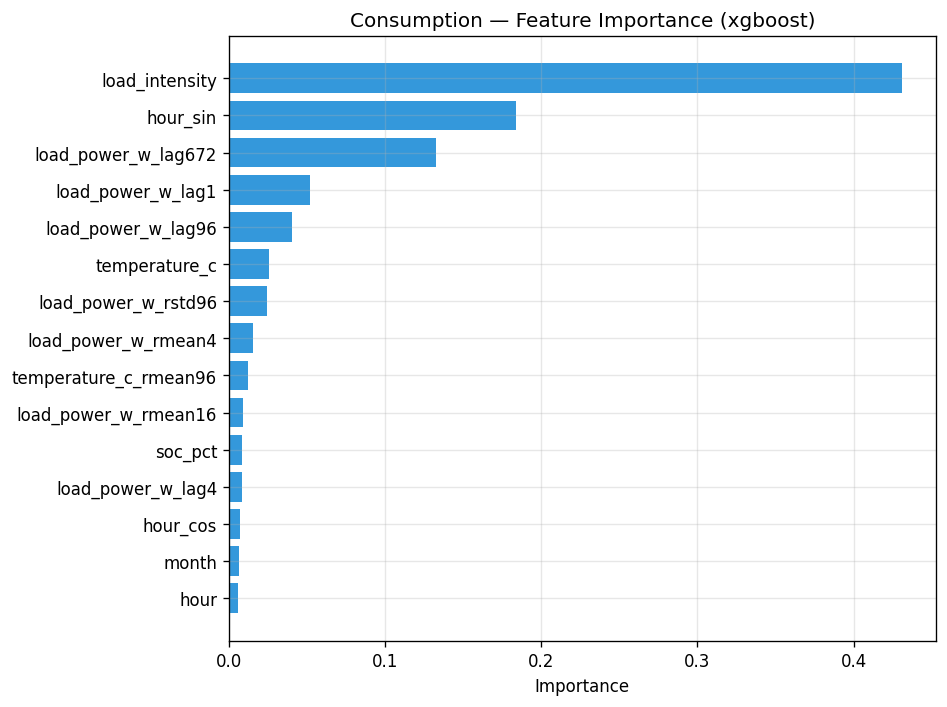
\includegraphics[width=0.75\textwidth]{figures/consumption_features.png}
    \caption{XGBoost feature importance for consumption forecasting.}
    \label{fig:feature_importance}
\end{figure}

For the consumption XGBoost model, the five most important features are:
\begin{enumerate}[nosep]
    \item \texttt{load\_power\_w\_lag1} --- previous time step consumption
    \item \texttt{load\_power\_w\_lag96} --- same time yesterday
    \item \texttt{hour\_sin} / \texttt{hour\_cos} --- time of day
    \item \texttt{temperature\_c} --- ambient temperature (correlates with AC usage)
    \item \texttt{load\_power\_w\_rmean4} --- 1-hour rolling mean
\end{enumerate}

The dominance of lag features confirms that short-term autocorrelation drives the forecast, while temperature captures the AC-driven seasonal component.
